Facciamo ora un riassunto delle forze coinvolte nei processi di dissoluzione.

Le forze intermolecolari sono attrazioni intermolecolari che si esercitano tra atomi, molecole o ioni. Parleremo di ioni quando avremo a che fare con elettroliti, mentre parleremo di molecole quando avremo soluzioni di non elettroliti, ad esempio acqua e saccarosio. Infine parleremo di atomi quando avremo a che fare con soluzioni di specie atomiche.
\subsection{Forze ione-ione}
Sono le interazioni più forti. Si esercitano tra ioni di carica opposta e tale forza è la forza di Coulomb:

\begin{minipage}{0.5 \textwidth}
    \vspace{1cm}
    $$F \propto \frac{q_1 \cdot q_2}{d^2}$$
\end{minipage}
\begin{minipage}{0.5 \textwidth}
    \begin{figure}[H]
        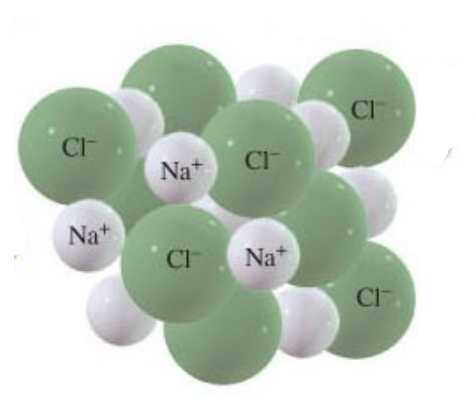
\includegraphics[width=4cm]{immagini/forze_ione_ione.png}
    \end{figure}
\end{minipage}

\subsection{Forze ione-dipolo}
L'acqua è una molecola dipolare, cioè ha un forte momento di dipolo. Pertanto sono queste le forze in gioco nei processi di dissoluzione degli elettroliti o di solidi ionici. La forza cioè sarà proporzionale al prodotto della carica del singolo ione per il momento di dipolo della molecola in questione, come ad esempio l'acqua:

\begin{minipage}{0.5 \textwidth}
    \vspace{0.2cm}
    $$F \propto \frac{q \cdot \mu}{d^2}$$
\end{minipage}
\begin{minipage}{0.5 \textwidth}
    \begin{figure}[H]
        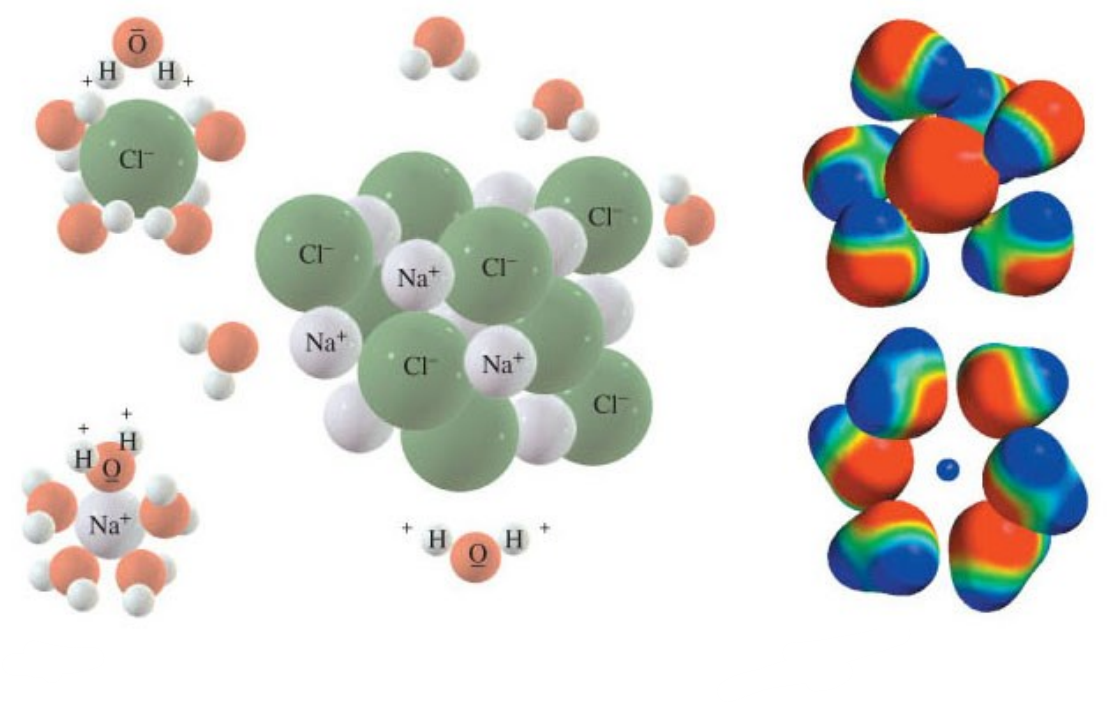
\includegraphics[width=7cm]{immagini/forze_ione_dipolo.png}
    \end{figure}
\end{minipage}

\subsection{Forze dipolo-dipolo}
Abbiamo visto il legame ad idrogeno. Più in generale le forze che si esercitano tra molecole che possiedono momenti di dipolo permanenti sono forze date dal prodotto dei momenti di dipolo diviso la distanza al cubo:

$$F \propto \frac{\mu_1 \cdot \mu_2}{d^3}$$

Tali forze si hanno sia se le molecole dotate di momento di dipolo sono uguali sia se sono diverse, come nel caso di acqua e metanolo CH$_3$OH. In questo caso l'idrogeno legato all'ossigeno del metanolo interagisce con l'ossigeno di una molecola d'acqua. Non interagiscono gli altri tre perché il legame carbonio-idrogeno è poco polare a differenza di quello carbonio-ossigeno. Infatti la carica di questo legame è fortemente spostata verso l'ossigeno, quindi solo l'idrogeno legato all'ossigeno può interagire con l'ossigeno di una molecola d'acqua (grazie alla forte carica parziale positiva sull'idrogeno), e può quindi formare un legame ad idrogeno con l'ossigeno dell'acqua.

\hspace{0.5cm}\begin{minipage}{0.35 \textwidth}
    \begin{figure}[H]
        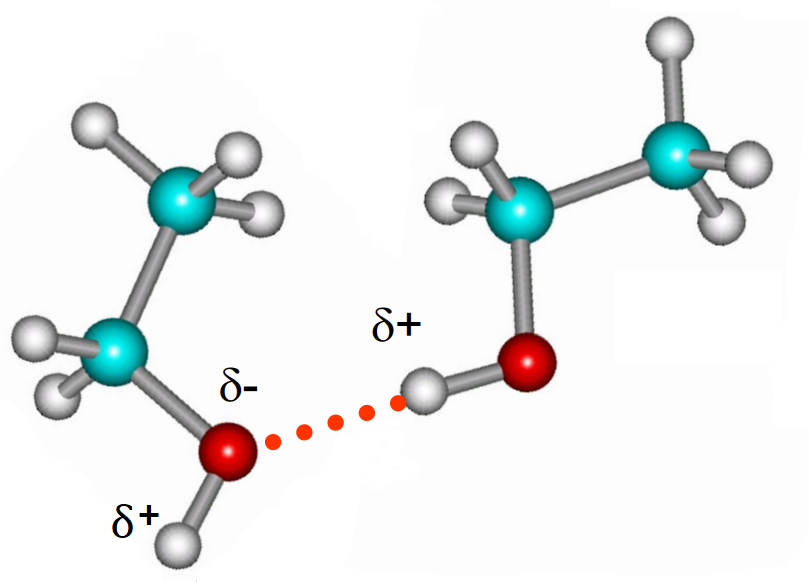
\includegraphics[width=5cm]{immagini/alcol_etilico.png}
    \end{figure}
\end{minipage}
\begin{minipage}{0.6 \textwidth}
    \vspace{0.6cm}Un altro esempio sono due molecole di alcol etilico CH$_3$CH$_2$OH. Anche qui i legami carbonio-idrogeno sono debolmente polari, mentre il legame carbonio-ossigeno è polare. Ecco quindi che l'idrogeno del gruppo OH di una molecola interagirà con l'ossigeno del gruppo OH di un'altra molecola, instaurando un legame.
\end{minipage}

\hspace{0.5cm}\begin{minipage}{0.35 \textwidth}
    \begin{figure}[H]
        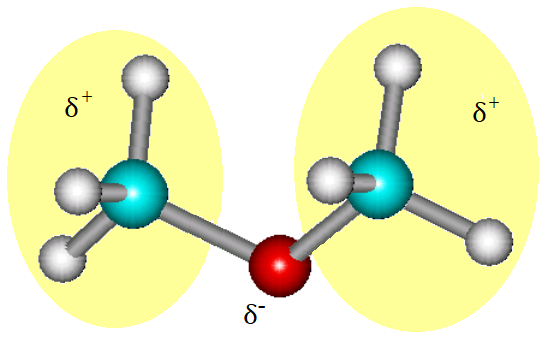
\includegraphics[width=5cm]{immagini/etere_dimetilico.png}
    \end{figure}
\end{minipage}
\begin{minipage}{0.6 \textwidth}
    \vspace{0.6cm}L'etere dimetilico (CH$_3$OCH$_3$) è un'altra molecola che può formare legami polari coinvolti in interazioni ad idrogeno. In questa molecola, l'ossigeno ha una parziale carica negativa perché i gruppi metilici CH$_3$ risultano positivizzati dall'elettronegatività dell'ossigeno che porta questo ad attirare su di sé carica negativa che sottrae a tali gruppi. In questa molecola il momento di dipolo è ancora più basso perché fondamentalmente abbiamo interazioni carbonio-ossigeno.
\end{minipage}

\vspace{0.2cm}I legami a idrogeno sono inoltre responsabili dell'alto punto di ebollizione di alcune specie.

\hspace{0.5cm}\begin{minipage}{0.35 \textwidth}
    \begin{figure}[H]
        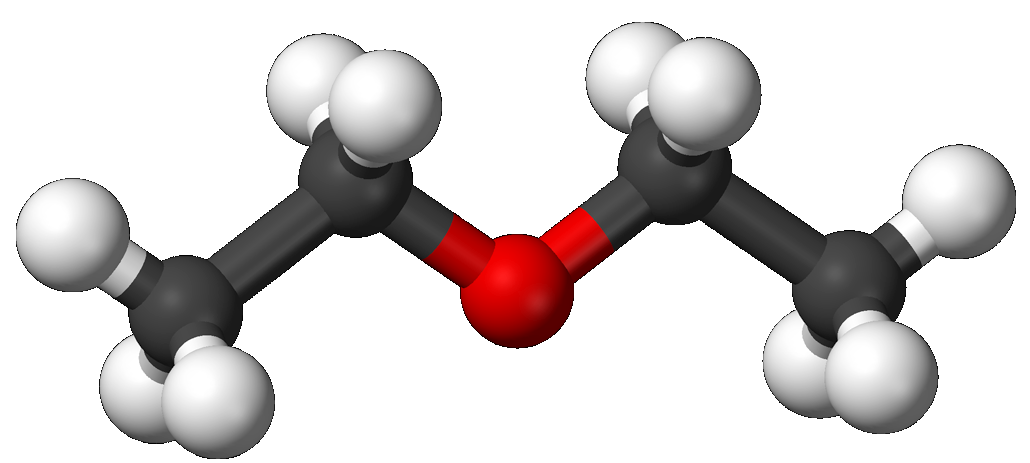
\includegraphics[width=5cm]{immagini/etere_dietilico.png}
    \end{figure}
\end{minipage}
\begin{minipage}{0.6 \textwidth}
    \vspace{0.6cm}Se infine consideriamo l'etere dietilico C$_2$H$_5$OC$_2$H$_5$, questa molecola ha un momento maggiore e un punto di fusione maggiore di quelli dell'etere dimetilico. Ciò avviene perché i legami a idrogeno non sono l'unica interazione debole che determina momenti di dipolo e punti di ebollizione. Nel caso particolare, fra le catene laterali possono esercitarsi alcuni tipi di interazioni dette di \textit{Van der Waals}.
\end{minipage}

\vspace{0.2cm}Quindi quando si cerca di portare ad ebollizione un composto, la massa del composto ha un ruolo importante, ma non bisogna sottovalutare l'importanza delle interazioni da rompere fra le singole molecole (A-A se è una specie chimica, A-B se è una soluzione di A e B), qualora si instaurino.

\subsection{Forze ione-dipolo indotto o dipolo-dipolo indotto}
Alcune molecole non hanno un momento di dipolo permanente a causa della distribuzione uniforme delle cariche elettriche all'interno della molecola. Tuttavia, quando queste molecole vengono avvicinate a una specie carica, come ad esempio un ione o una molecola polarizzata, si può generare un momento di dipolo indotto nella molecola. Quello che succede è che la nube elettronica viene distorta, generando una separazione di cariche. 

Sotto forma di simboli avremo

\begin{figure}[htp]
    \centering
    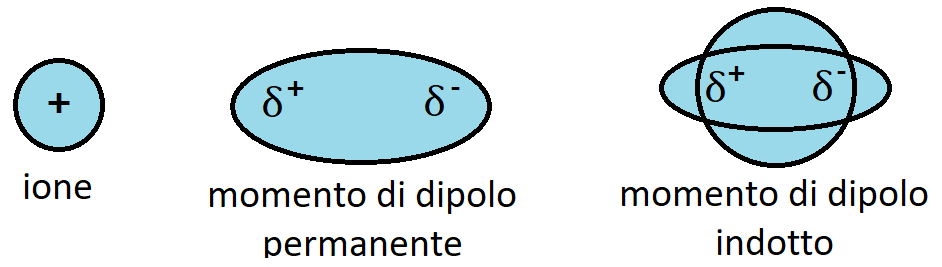
\includegraphics[width=11cm]{immagini/ioni_e_momenti_di_dipolo.png}
\end{figure}

Ci sono infine anche delle \textbf{forze dipolo indotto-dipolo indotto} che prendono il nome di \textit{Forze di London o di dispersione}.

In tutto questi casi le forze esercitate hanno l'andamento di $1/d^6$.
\subsection{La viscosità}
Le interazioni di Van der Waals e le interazioni ad idrogeno sono due classi di forze intermolecolari che determinano la viscosità di un liquido, ovvero la sua resistenza al flusso (come attrito interno). La viscosità non è da confondere con la densità del liquido, che invece è una proprietà intrinseca della materia.

Le interazioni ad idrogeno sono relativamente deboli e possono essere facilmente rotte, ad esempio riscaldando il liquido. Quando ciò avviene, anche le interazioni di Van der Waals vengono meno, poiché dipendono in gran parte dalla distanza tra le molecole. Di conseguenza, la viscosità del liquido diminuisce all'aumentare della temperatura, poiché le forze che determinano la resistenza al flusso sono meno efficaci. Questo è uno dei motivi per cui i liquidi diventano più fluidi a temperature elevate, come ad esempio l'olio da cucina quando lo si scalda sulla stufa.